\chapter{Παραγωγή Codebooks}
\label{chapter:chap4}

\section{Εισαγωγή}
\label{section:sect41}

\indent Σε αυτό το κεφάλαιο θα παρουσιαστεί ο τρόπος με τον οποίο εκπαιδεύτηκε ο kmeans (training) και με ποία δεδομένα (training set). Επίσης θα δειχθεί ο τρόπος εξαγωγείς των δεδομένων από τον H.264.

\section{Επιλογή του training set}
\label{section:sect42}

\indent Όπως εξηγήθηκε στο Κεφάλαιο~\ref{chapter:chap2} τα δεδομένα που ένας κωδικοποιητής συμπιέζει είναι τα residuals και όχι τα pixels. Πρέπει να είναι ξεκάθαρο πως τα residuals μαζί με τα motion vector μας δίνουν όλη την πληροφορία για να ανακατασκευάσουμε ένα καρέ. Αν δεν έχει παρεμβληθεί η κβαντοποίηση τότε το ανακατασκευασμένο με το αυθεντικό καρέ θα είναι πανομοιότυπα. Έτσι λοιπόν επιλέχθηκαν τα residuals να είναι το training set του kmeans.

\indent Μέχρι τώρα έχει γίνει σαφές πως για κάθε καρέ διάστασης W*H pixels υπάρχουν W*H residuals. Επομένως είναι εφικτό να τεμαχίσουμε το καρέ σε d*d blocks οπού d η διάσταση του training set. Το d έχει τον μοναδικό περιορισμό ότι πρέπει να είναι μικρότερο από την διάσταση του block του encoder, στον H.264 που αυτή η διπλωματική βασίστηκε $blocksize\in[2*2,16*16]$ και μπορεί να ρυθμιστεί ανάλογα. Η διάσταση που επιλέχθηκε είναι το $d=4$ που πληρεί το κριτήριο "blocksize" και είναι η προεπιλεγμένη τιμή blocksize στον H.264. Έστω ένα καρέ ανάλυσης 720*480 με YUV420 τότε συνολικά έχουμε $720*480*1.5=518400$ pixels και $ \frac{518400}{4*4} = 32400 $ training vectors.

\indent Τα βίντεο που θα μας έδινα το training set έπρεπε να επιλεχθούν προσεκτικά γιατί χρειάζεται να πληρούν κάποιες προϋποθέσεις.
\begin{itemize}
    \item Θα πρέπει να υπάρχει ένας ικανοποιητικός αριθμός από καρέ για να μπορέσουμε να έχουμε αντιπροσωπευτικά στατιστικά. Στην διπλωματική χρησιμοποιήθηκαν 2600 καρέ από 10 διαφορετικά βίντεο ανάλυσης 720*480. Αρά συνολικά είχαμε 84240000 training vectors που θεωρείται ικανοποιητικός αριθμός.
    \item Το περιεχόμενο των βίντεο παίζει καθοριστικό ρόλο για το PSNR του VQ όταν δοκιμάζετε σε βίντεο εκτός του training set. Για παράδειγμα εάν το training set μας δε περιλαμβάνει σκηνές που απεικονίζουν βουνά τότε αν κωδικοποιηθεί ένα βίντεο που περιέχει σκηνές από βουνά θα έχουμε χαμηλά PSNR (φαινόμενο mismatch). Τα 10 βίντεο που χρησιμοποιήθηκαν είχαν διαφορετικές σκηνές και μπορούμε να δούμε κάποια στιγμιότυπα στο Σχήμα~\ref{fig:trainingset}.
\end{itemize}

\indent Θεωρητικά το καλύτερο training set θα ήταν όλα τα βίντεο που κυκλοφορούν στον πλανήτη (talk shows, ταινίες, αθλήματα κ.τ.λ) αλλά τότε η πολυπλοκότητα του προβλήματος αυξάνεται σε επίπεδα που οι σημερινοί υπολογιστές δεν μπορούν να λύσουν σε εύλογο χρονικό διάστημα.

\begin{figure}[p]
\centering
\begin{tabular}{c c}
    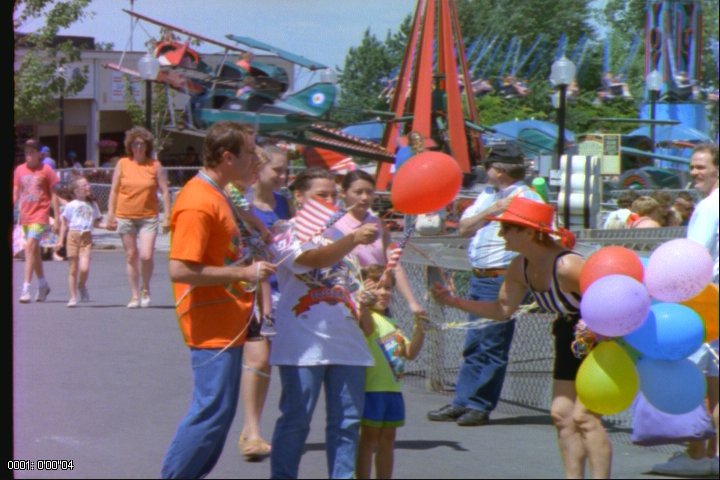
\includegraphics[height=4.0cm]{chapter4/frames/src13.png}
    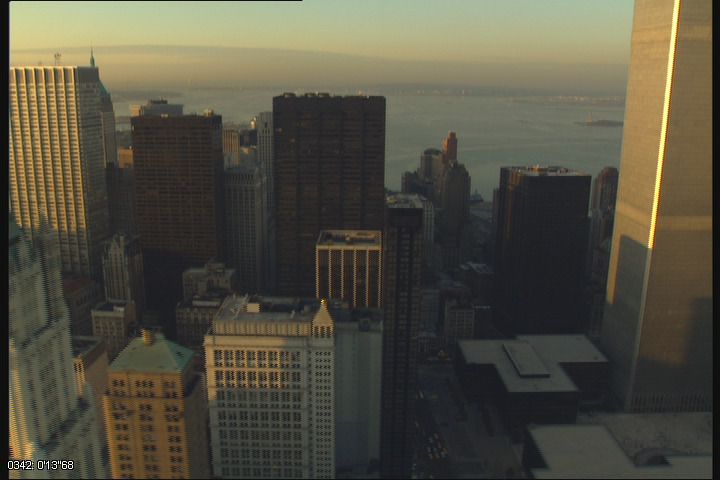
\includegraphics[height=4.0cm]{chapter4/frames/src14.png}\\
    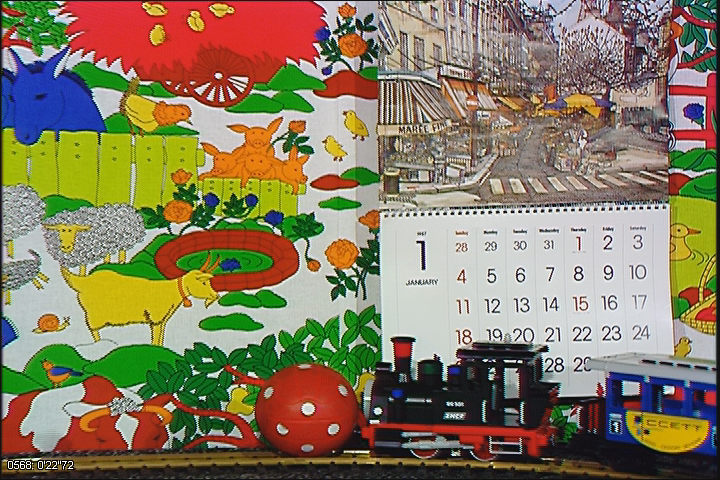
\includegraphics[height=4.0cm]{chapter4/frames/src15.png}
    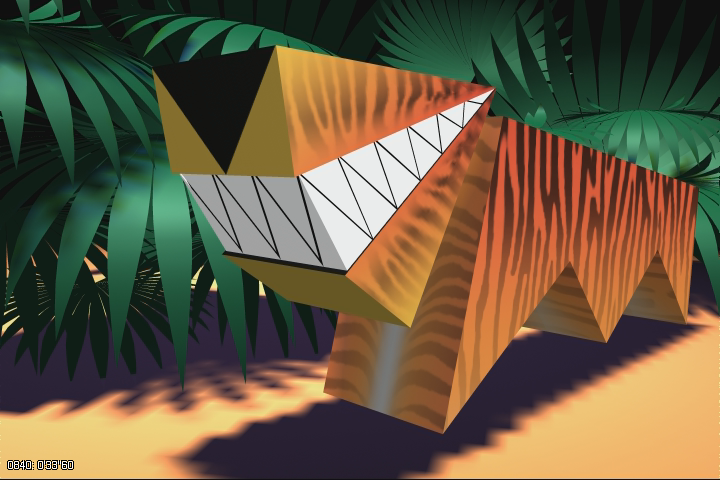
\includegraphics[height=4.0cm]{chapter4/frames/src16.png}\\
    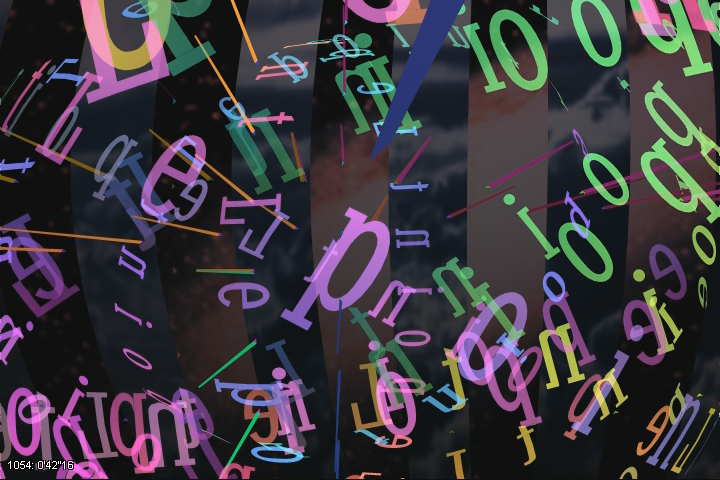
\includegraphics[height=4.0cm]{chapter4/frames/src17.png}
    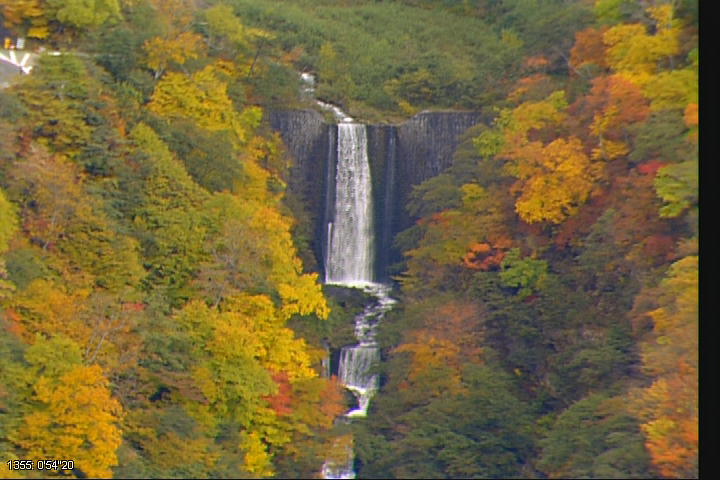
\includegraphics[height=4.0cm]{chapter4/frames/src18.png}\\
    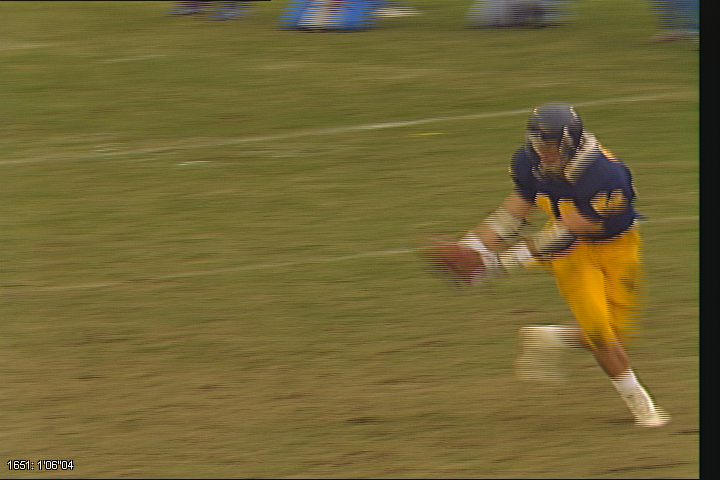
\includegraphics[height=4.0cm]{chapter4/frames/src19.png}
    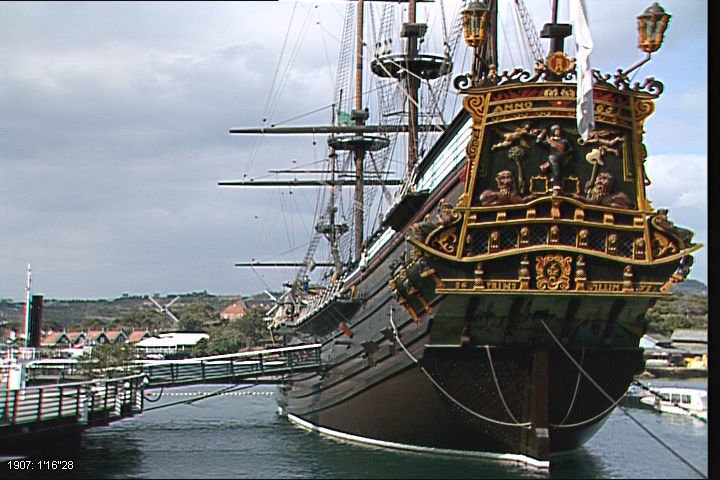
\includegraphics[height=4.0cm]{chapter4/frames/src20.png}\\
    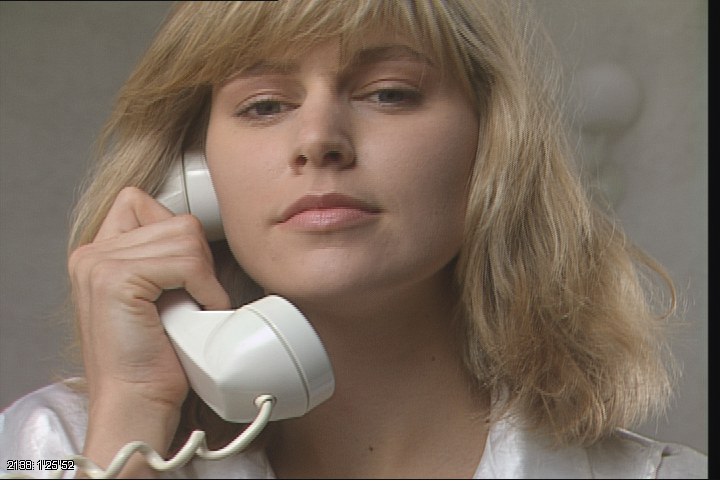
\includegraphics[height=4.0cm]{chapter4/frames/src21.png}
    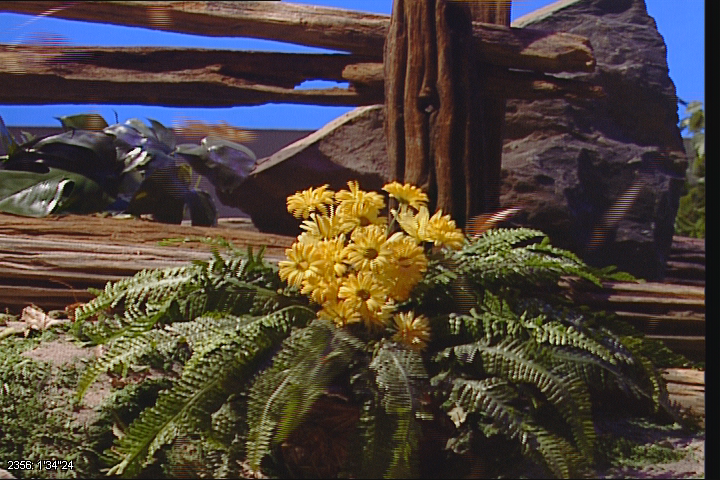
\includegraphics[height=4.0cm]{chapter4/frames/src22.png}
\end{tabular}
\caption{Training βίντεο.}
\label{fig:trainingset}
\end{figure}

\newpage

\section{Εξαγωγή training set από τον H.264}
\label{section:sect43}

\indent Η εξαγωγή των residuals από τον H.264 έγινε από τον decoder και όχι από τον encoder. Αυτή η επιλογή έγινε γιατί ο κώδικας του encoder είναι πιο περίπλοκος απο αυτόν του decoder. Επίσης αναφέρθηκε στο Κεφάλαιο~\ref{chapter:chap2} ότι ο encoder κάνει δοκιμές για να βρει το καλύτερο Intra Prediction Mode αν τα καρέ είναι I,P,B είναι ψάχνει να βρει σε προηγούμενα/επομένα καρέ το καλύτερο match ώστε να βγάλει το Motion Vector. Η παραπάνω διαδικασία δυσκόλεψε τον εντοπισμό του σημείου που βρίσκονται τα residuals του καλύτερου mode.

\indent Στον decoder η διαδικασία ήταν αρκετά απλή. Απλά έπρεπε να βρεθεί το σημείο που ο decoder αποκωδικοποιεί τα macroblocks, τα residuals/macroblock σε αυτό το σημείο ήταν εύκολα προσβάσιμα. Στην συνέχεια το macroblock διάστασης 16x16 με τα residuals χωρίζονταν σε block διάστασης dxd και γράφονταν στο αρχείο όπως φαίνεται στο Σχήμα~\ref{fig:storeres}. Το επόμενο που έγινε είναι να μπορεί να χωρίζει τα vectors σε I,P,B και να τα γράφει σε ξεχωριστά αρχεία καθώς επίσης και να ξεχωρίζει τα Y,UV. Ακόμα ένα στοιχείο που προστέθηκε είναι να υπάρχει η δυνατότητα να εξαχθεί ολόκληρο καρέ διάστασης όσο το βίντεο εισόδου. Τέλος το configuration file του JM H.264 τροποποιήθηκε έτσι ώστε να μπορούμε να δώσουμε τις παρακάτω επιλογές.

\begin{itemize}
    \item ResidualsFileY το αρχείο εξόδου των residuals του Υ.
    \item ResidualsFileUV το αρχείο εξόδου των residuals του UV.
    \item ResidualsDims η διάσταση των residuals.
    \item KeepI,B,P διακόπτες που ενεργοποιούν την εξαγωγή μόνο τον I,P,B αντίστοιχα.
    \item ResidualsMode αν είναι 0 τότε δεν γίνετε καθόλου εξαγωγή. Αν είναι 1 τότε γίνετε εξαγωγή για είσοδο στον kmeans. Αν είναι 2 γίνετε εξαγωγή ολόκληρων καρέ.
\end{itemize}

\indent Αφού η διαδικασία γίνετε στον decoder θα έπρεπε αρχικά να συμπιέσουμε το βίντεο. Η συμπίεση που έγινε ήταν σε lossless mode με την λειτουργία FRExT του H.264 γιατί στον decoder θέλαμε τα residuals χωρίς θόρυβο. Η συμπίεση έγινε δύο φορές με δύο διαφορετικά GOP και έγινε τρεις φόρες αποσυμπίεση μια για κάθε mode.

\begin{itemize}
    \item Για να παραχθεί το I training set συμπιέσαμε τα 2600 καρέ με GOP I-I-I-.... και αποσυμπιέσαμε με KeepI=1 και ResidualsMode=1.
    \item Για να παραχθεί το P training set συμπιέσαμε τα 2600 καρέ με GOP I-P-P-B-P-P-B.... και αποσυμπιέσαμε με KeepP=1 και ResidualsMode=1.
    \item Για να παραχθεί το B training set συμπιέσαμε τα 2600 καρέ με GOP I-P-P-B-P-P-B.... και αποσυμπιέσαμε με KeepB=1 και ResidualsMode=1. Αλλά είδαμε πως τα vectors που ήταν πραγματικά Bidirectional ήταν λίγα και δεν αρκούσαν για΄να εξαχθούν στατιστικά. Επομένως θέσαμε και το KeepP=1 έτσι ώστε να συμπεριληφθούν όλα τα Inter vectors.
\end{itemize}

\indent Συνεπώς παράχθηκαν 4 training set τα Intra Y,Intra UV,Inter Y,Inter UV διάστασης 16 και πλήθους αρκετά μεγάλου ώστε να μπορούν να εξαχθούν καλά codebooks.

\section{Kmeans}
\label{section:sect44}

\indent Ο kmeans εφαρμόστηκε στα training set που φαίνονται στον Πίνακα~\ref{table:trainingset} και παρατηρούμε πως τα πειράματα έτρεχαν για 23 μέρες. Τα k=65536 επιλέχθηκε για να έχουμε VQ indeces στο διάστημα [0,65535] έτσι ώστε να χρειαζόμαστε ακριβώς 2 bytes για να αποθηκεύσουμε ένα index, επίσης βλέπουμε πως μας δίνει ένα PSNR κοντά στο βίντεο που θέλουμε να βλέπουμε στην καθημερινότητα μας. Η εντροπία είναι διαιρεμένη με την διάσταση οπότε αντιπροσωπεύει το κάθε residual.

\begin{table}[h!]
    \begin{center}
        \begin{tabular}{| l | l | l | l | l | l | l | l |}
        \hline
        Τύπος    & d  & Πλήθος   & k     & Εντροπία  & PSNR(dB) & Επαναλήψεις   & Διάρκεια\\ \hline
        IntraY   & 16 & 56160000 & 65536 & 0.712229  & 33.6     &  3249         & 12154                   \\ \hline
        IntraUV  & 16 & 28080000 & 65536 & 0.743071  & 42.1     &  2697         & 3119                    \\ \hline
        InterY   & 16 & 42117616 & 65536 & 0.692577  & 40.5     &  3270         & 9120                    \\ \hline
        InterUV  & 16 & 21058808 & 65536 & 0.707785  & 48.1     &  4221         & 8509                    \\ \hline
        \hline
        \end{tabular}
    \end{center}

    \caption{codebooks}
    \label{table:trainingset}
\end{table}

\section{Εντροπία υπό συνθήκη}
\label{section:sect45}

\indent Είναι γνωστό από την θεωρία Θεώρημα 2.6.5 [Cover] ότι αν έχουμε δύο τυχαίες μεταβλητές Χ,Υ τότε η πληροφορία που μα δίνει η Υ μπορεί μόνο να μειώσει την εντροπία της Χ, ισχύει δηλαδή πως $ H(X|Y=y_i) \leq H(X)$ με την ισότητα να ισχύει μόνο όταν Χ,Υ είναι ανεξάρτητες. Αυτό συμβαίνει μόνο όταν μπορούμε να έχουμε την πληροφορία για το Y χωρίς κάποιο επιπλέον κόστος. 

\indent Για να δοκιμαστεί αυτό το θεώρημα έγιναν τα παρακάτω βήματα. Παράχθηκε το κάθε training set με την μορφή καρέ τρέχοντας τον decoder με ResidualsMode=2. Για το συγκεκριμένο πείραμα αυτή η επιπλέον πληροφορία που δίνετε από την Υ είναι ο μέσος όρος της ενέργειας των ήδη κβαντισμένων block όπως φαίνεται στο Σχήμα~\ref{fig:averenergy}. Τα $y_i$ είναι περιοχές ενέργειας όπως φαίνεται στο Σχήμα~\ref{fig:cat}, παράχθηκαν ταξινομώντας με βάση την πιθανότητα τους τα clusters των codebooks και χωρίζοντας την ενέργεια σε οχτώ περιοχές με συνολικά ίση πιθανότητα. Ξεκινώντας από πάνω αριστερά κβαντοποιούνται τα block και κρατιούνται στατιστικά για το ποια είναι η κατηγορία του τρέχοντος block με βάση την ενέργεια τον γειτόνων του. Έτσι δημιουργούνται οχτώ νέες κατανομές πιθανότητας μεγέθους 65536, καθεμία μια από αυτές έχει δικιά της πιθανότητα.

\indent Αυτό το πείραμα με λίγα λογία λέει ότι αφού γνωρίζουμε την ενέργεια των κβαντοποιημένων block τότε ξέρουμε και την κατηγορία που ανήκει το τρέχων block. Έτσι κωδικοποιούμε (entropy encoding) με βάση την πιθανότητα του συγκεκριμένου cluster στην συγκεκριμένη κατηγορία ενέργειας. Το πείραμα πέτυχε καλύτερη εντροπία όπως φαίνεται στον Πίνακα~\ref{table:conentropy} σε σχέση με αυτήν του Πίνακα~\ref{table:trainingset} και αυτό συνέβη γιατί τα γειτονικά block μοιάζουν μεταξύ τους, άρα έχουν κοντινές ενέργειες. Επομένως έχουν μεγάλη εξάρτηση μεταξύ τους με κριτήριο την ενέργεια.

\begin{figure}[ht]
  \centering
  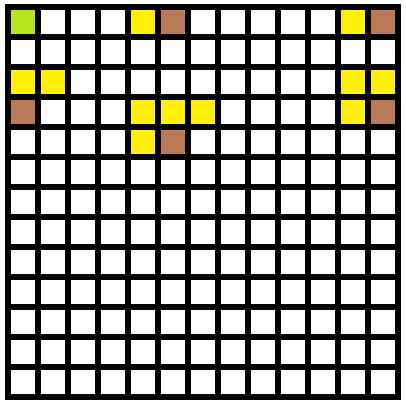
\includegraphics[width=0.5\textwidth]{chapter4/grid.png}
  \caption{Με καφέ είναι το τρέχων μπλοκ για κάθε περίπτωση και με κίτρινο από ποία γειτονικά βγαίνει ο μέσος όρος}
  \label{fig:averenergy}
\end{figure}

 \begin{figure}[h]
\centering
\begin{tabular}{c c}
    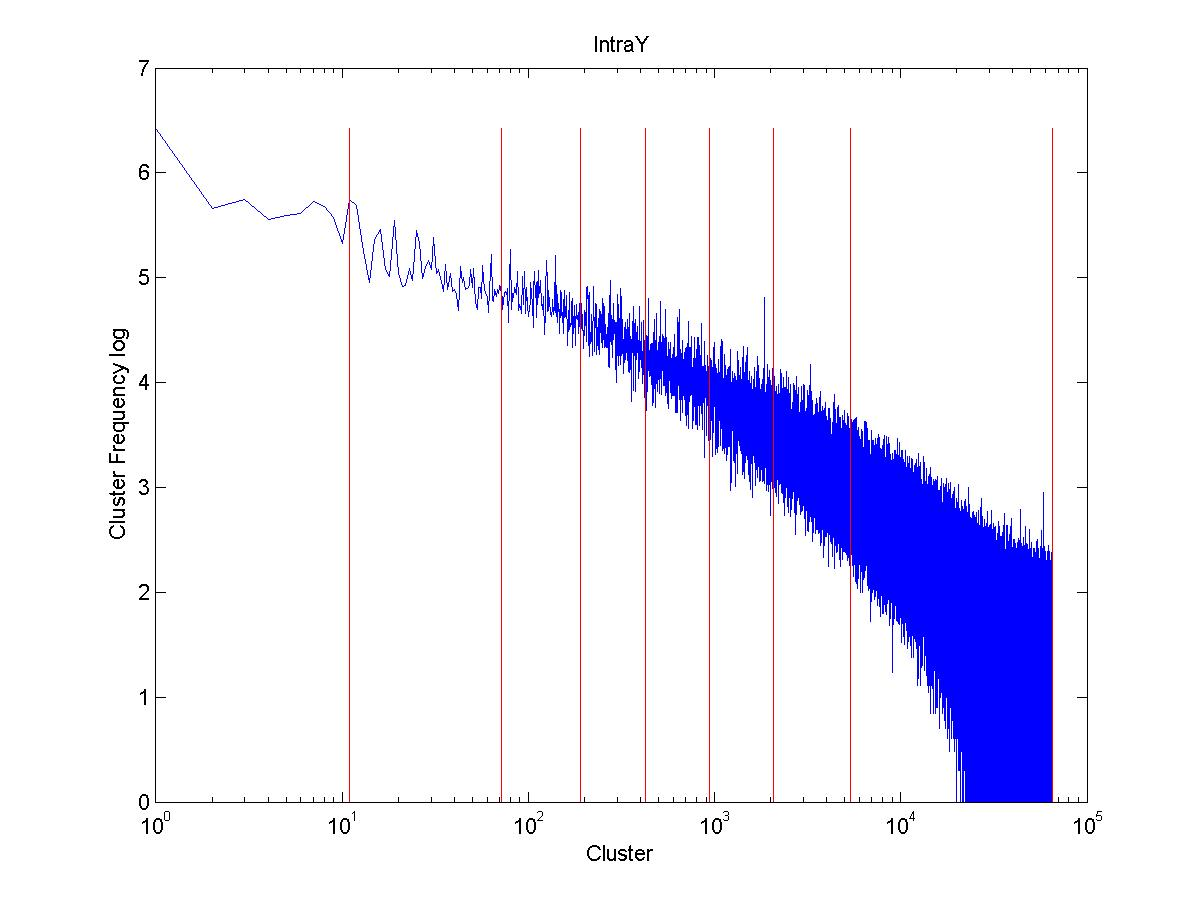
\includegraphics[height=6.0cm]{chapter4/IntraY.jpg}
    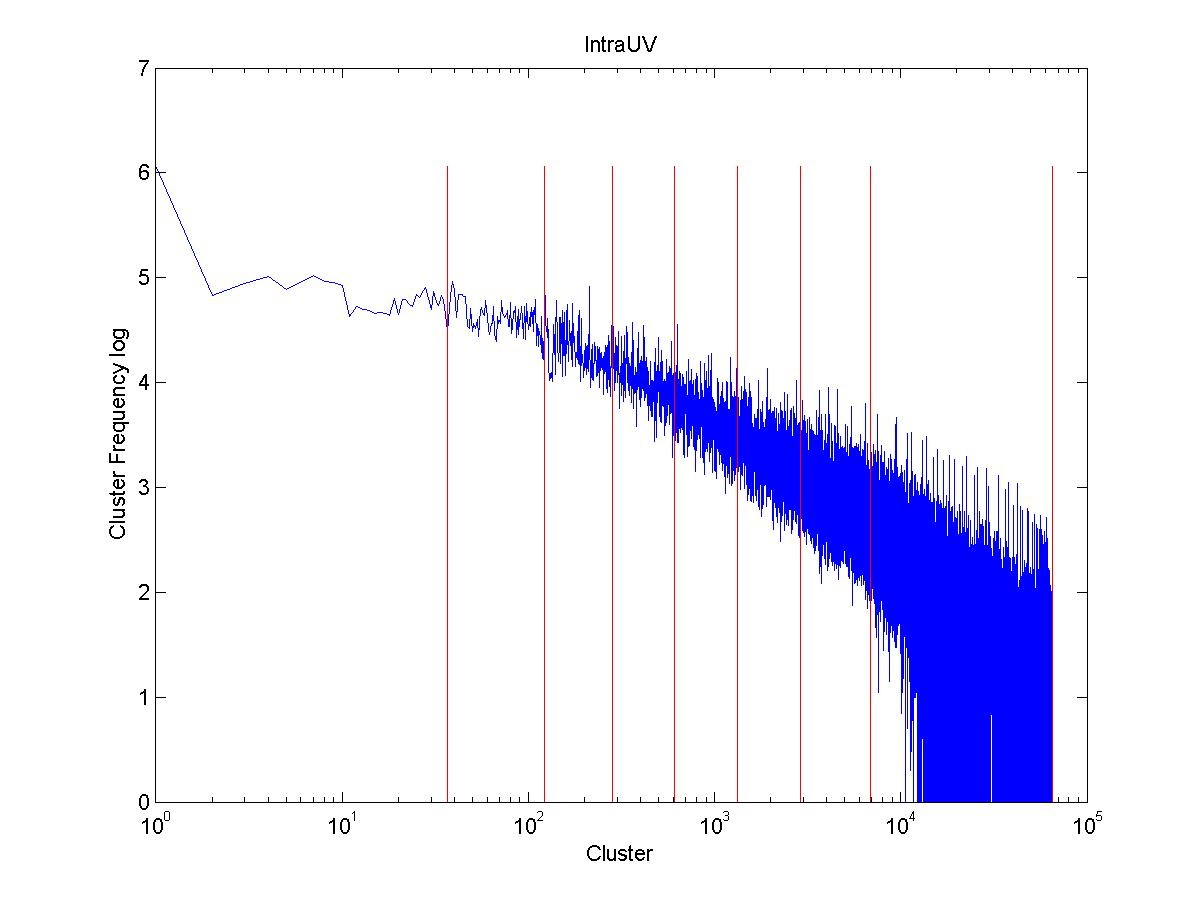
\includegraphics[height=6.0cm]{chapter4/IntraUV.jpg}\\
    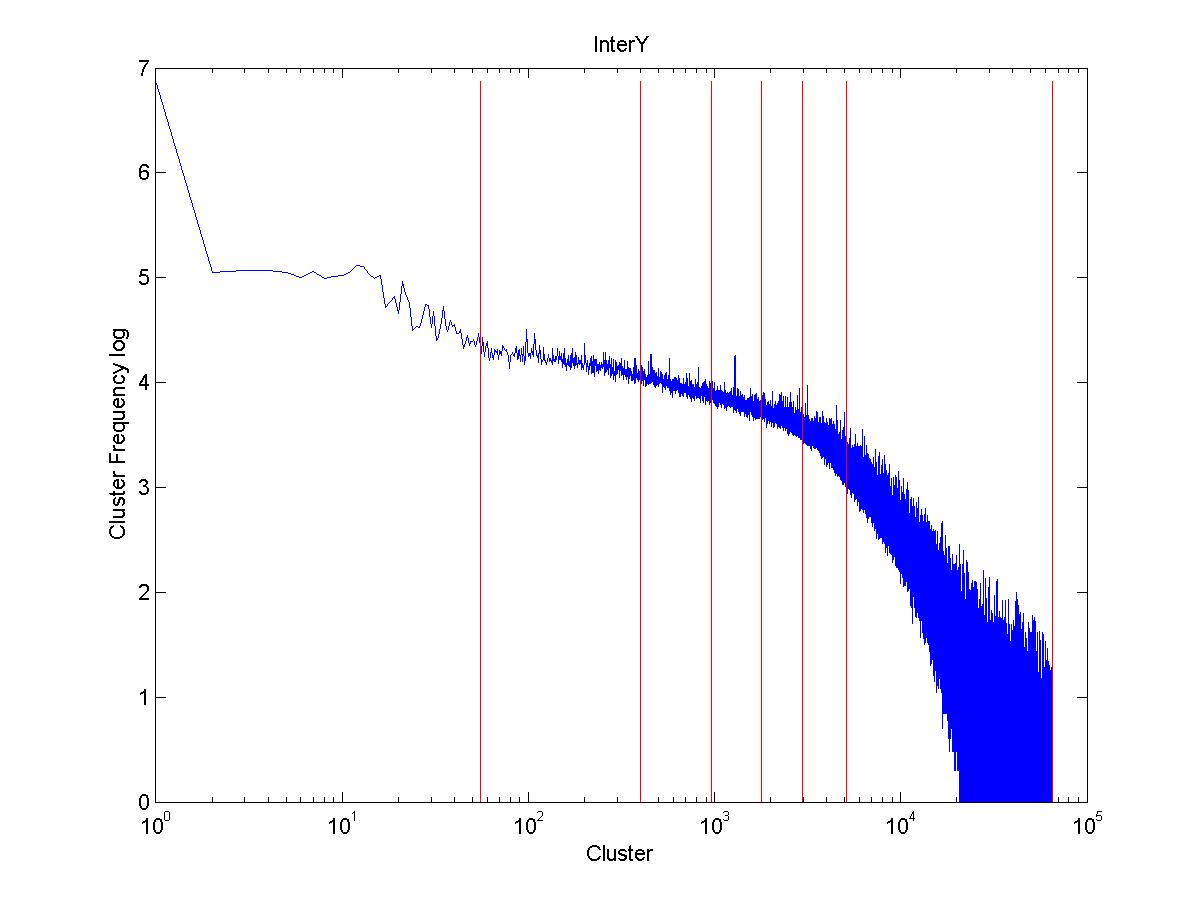
\includegraphics[height=6.0cm]{chapter4/InterY.jpg}
    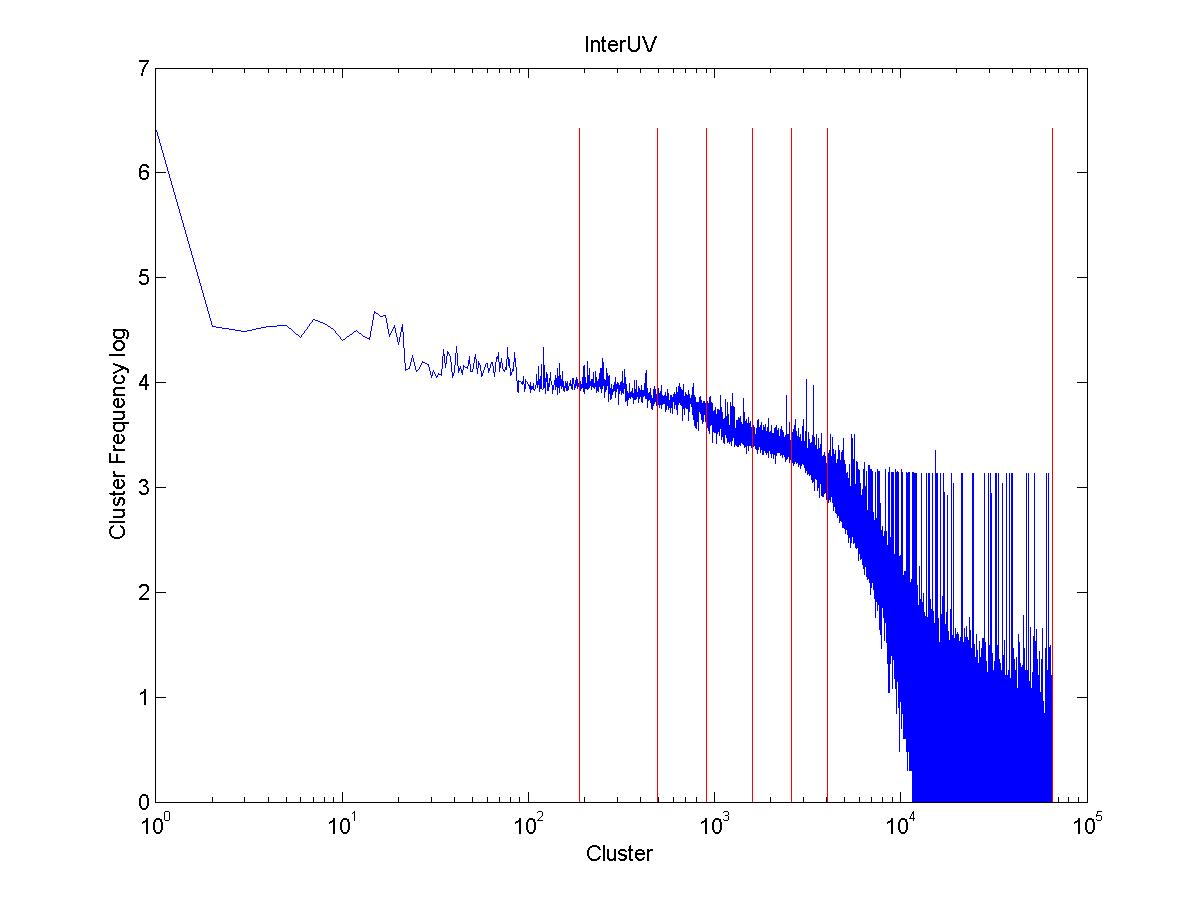
\includegraphics[height=6.0cm]{chapter4/InterUV.jpg}
\end{tabular}
\caption{Οι κόκκινες γραμμές δείχνουν το σημείο που σταματάει μια κατηγορία ενώ οι μπλε το πλήθος των vectors που αντιστοιχούν στο cluster}
\label{fig:cat}
\end{figure}

\begin{table}[h!]
    \begin{center}
        \begin{tabular}{| l | l | l | l | l | l | l | l |}
        \hline
        Τύπος    & Εντροπία \\ \hline
        IntraY   & 0.5      \\ \hline
        IntraUV  & 0.5      \\ \hline
        InterY   & 0.5      \\ \hline
        InterUV  & 0.5      \\ \hline
        \hline
        \end{tabular}
    \end{center}
    \caption{Εντροπία μετά την χρήση contexts}
    \label{table:conentropy}
\end{table} 